\chapter{Конструкторский раздел}
В данном разделе будут приведены схемы алгоритмов поиска заданного элемента в массиве методом линейного и бинарного поисков.

\section{Представление алгоритмов}

Алгоритмы на вход получают массив array, искомый элемент item. Возвращают индекс найденного элемента или иное значение, сигнализирующее об отсутствии искомого элемента в массиве. На рисунках \ref{fig:Liniar} --- \ref{fig:Binary} представлены схемы алгоритмов.

\begin{figure}[h]
	\centering
	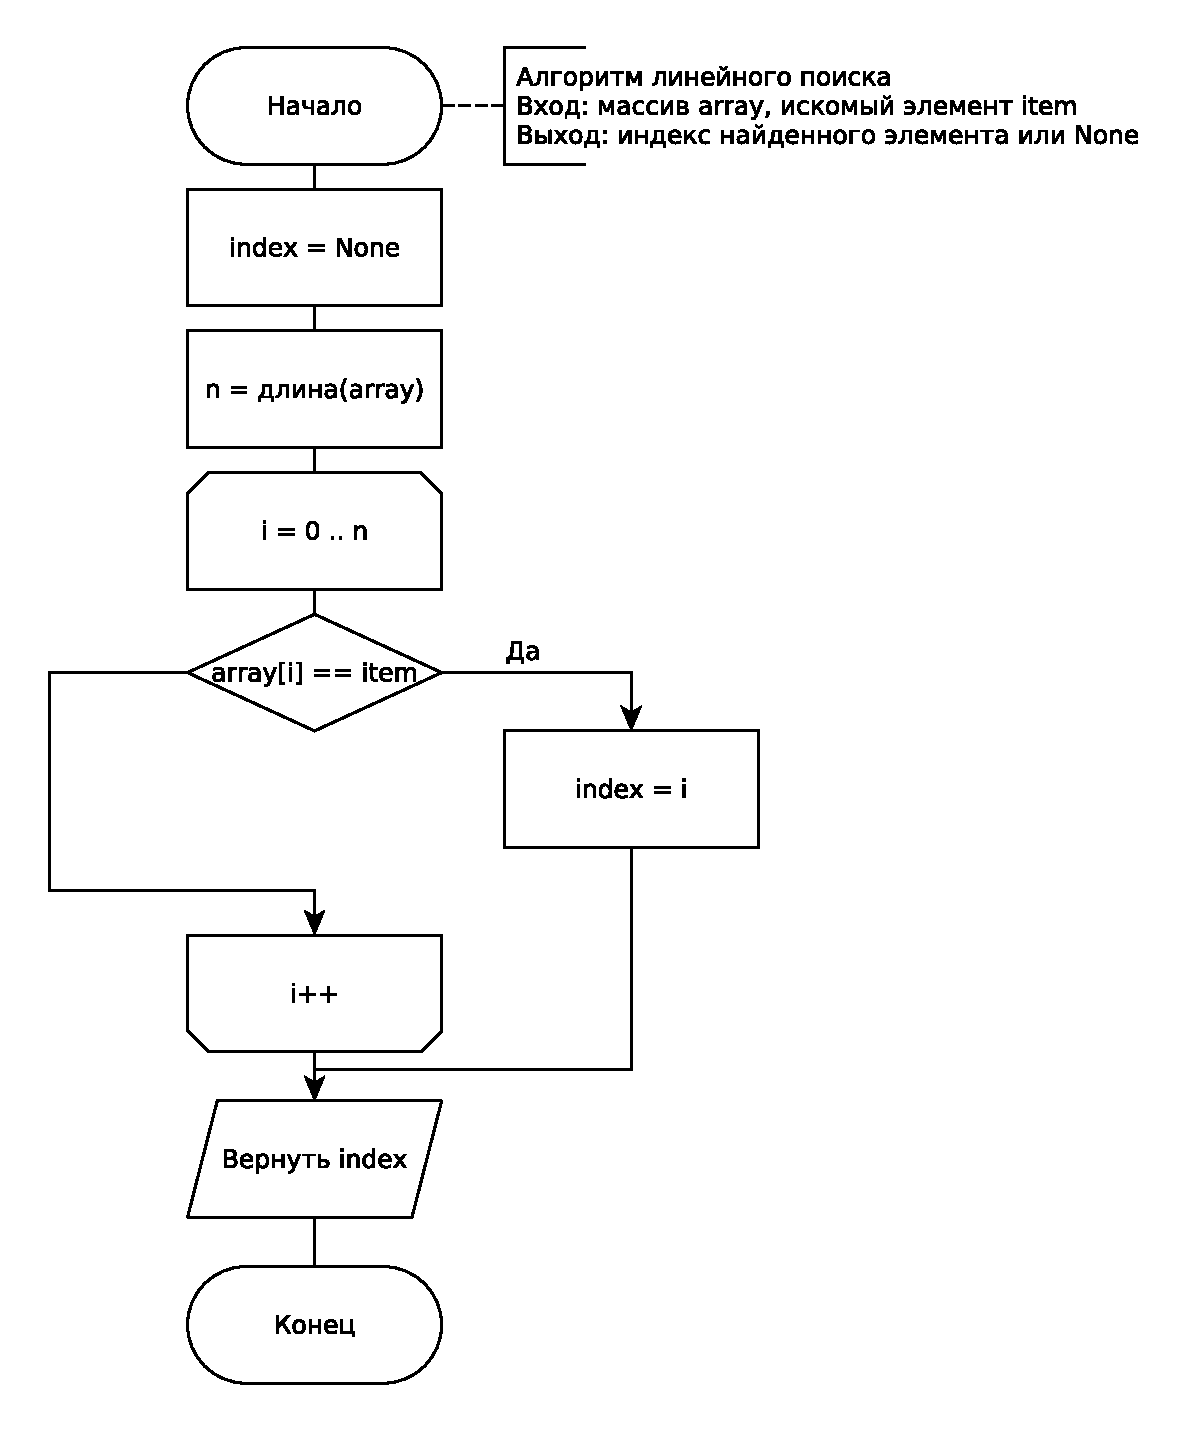
\includegraphics[scale=0.65]{img/liniar_search.eps}
	\caption{Схема алгоритма линейного поиска в массиве}
	\label{fig:Liniar}
\end{figure}

\clearpage

\begin{figure}
	\centering
	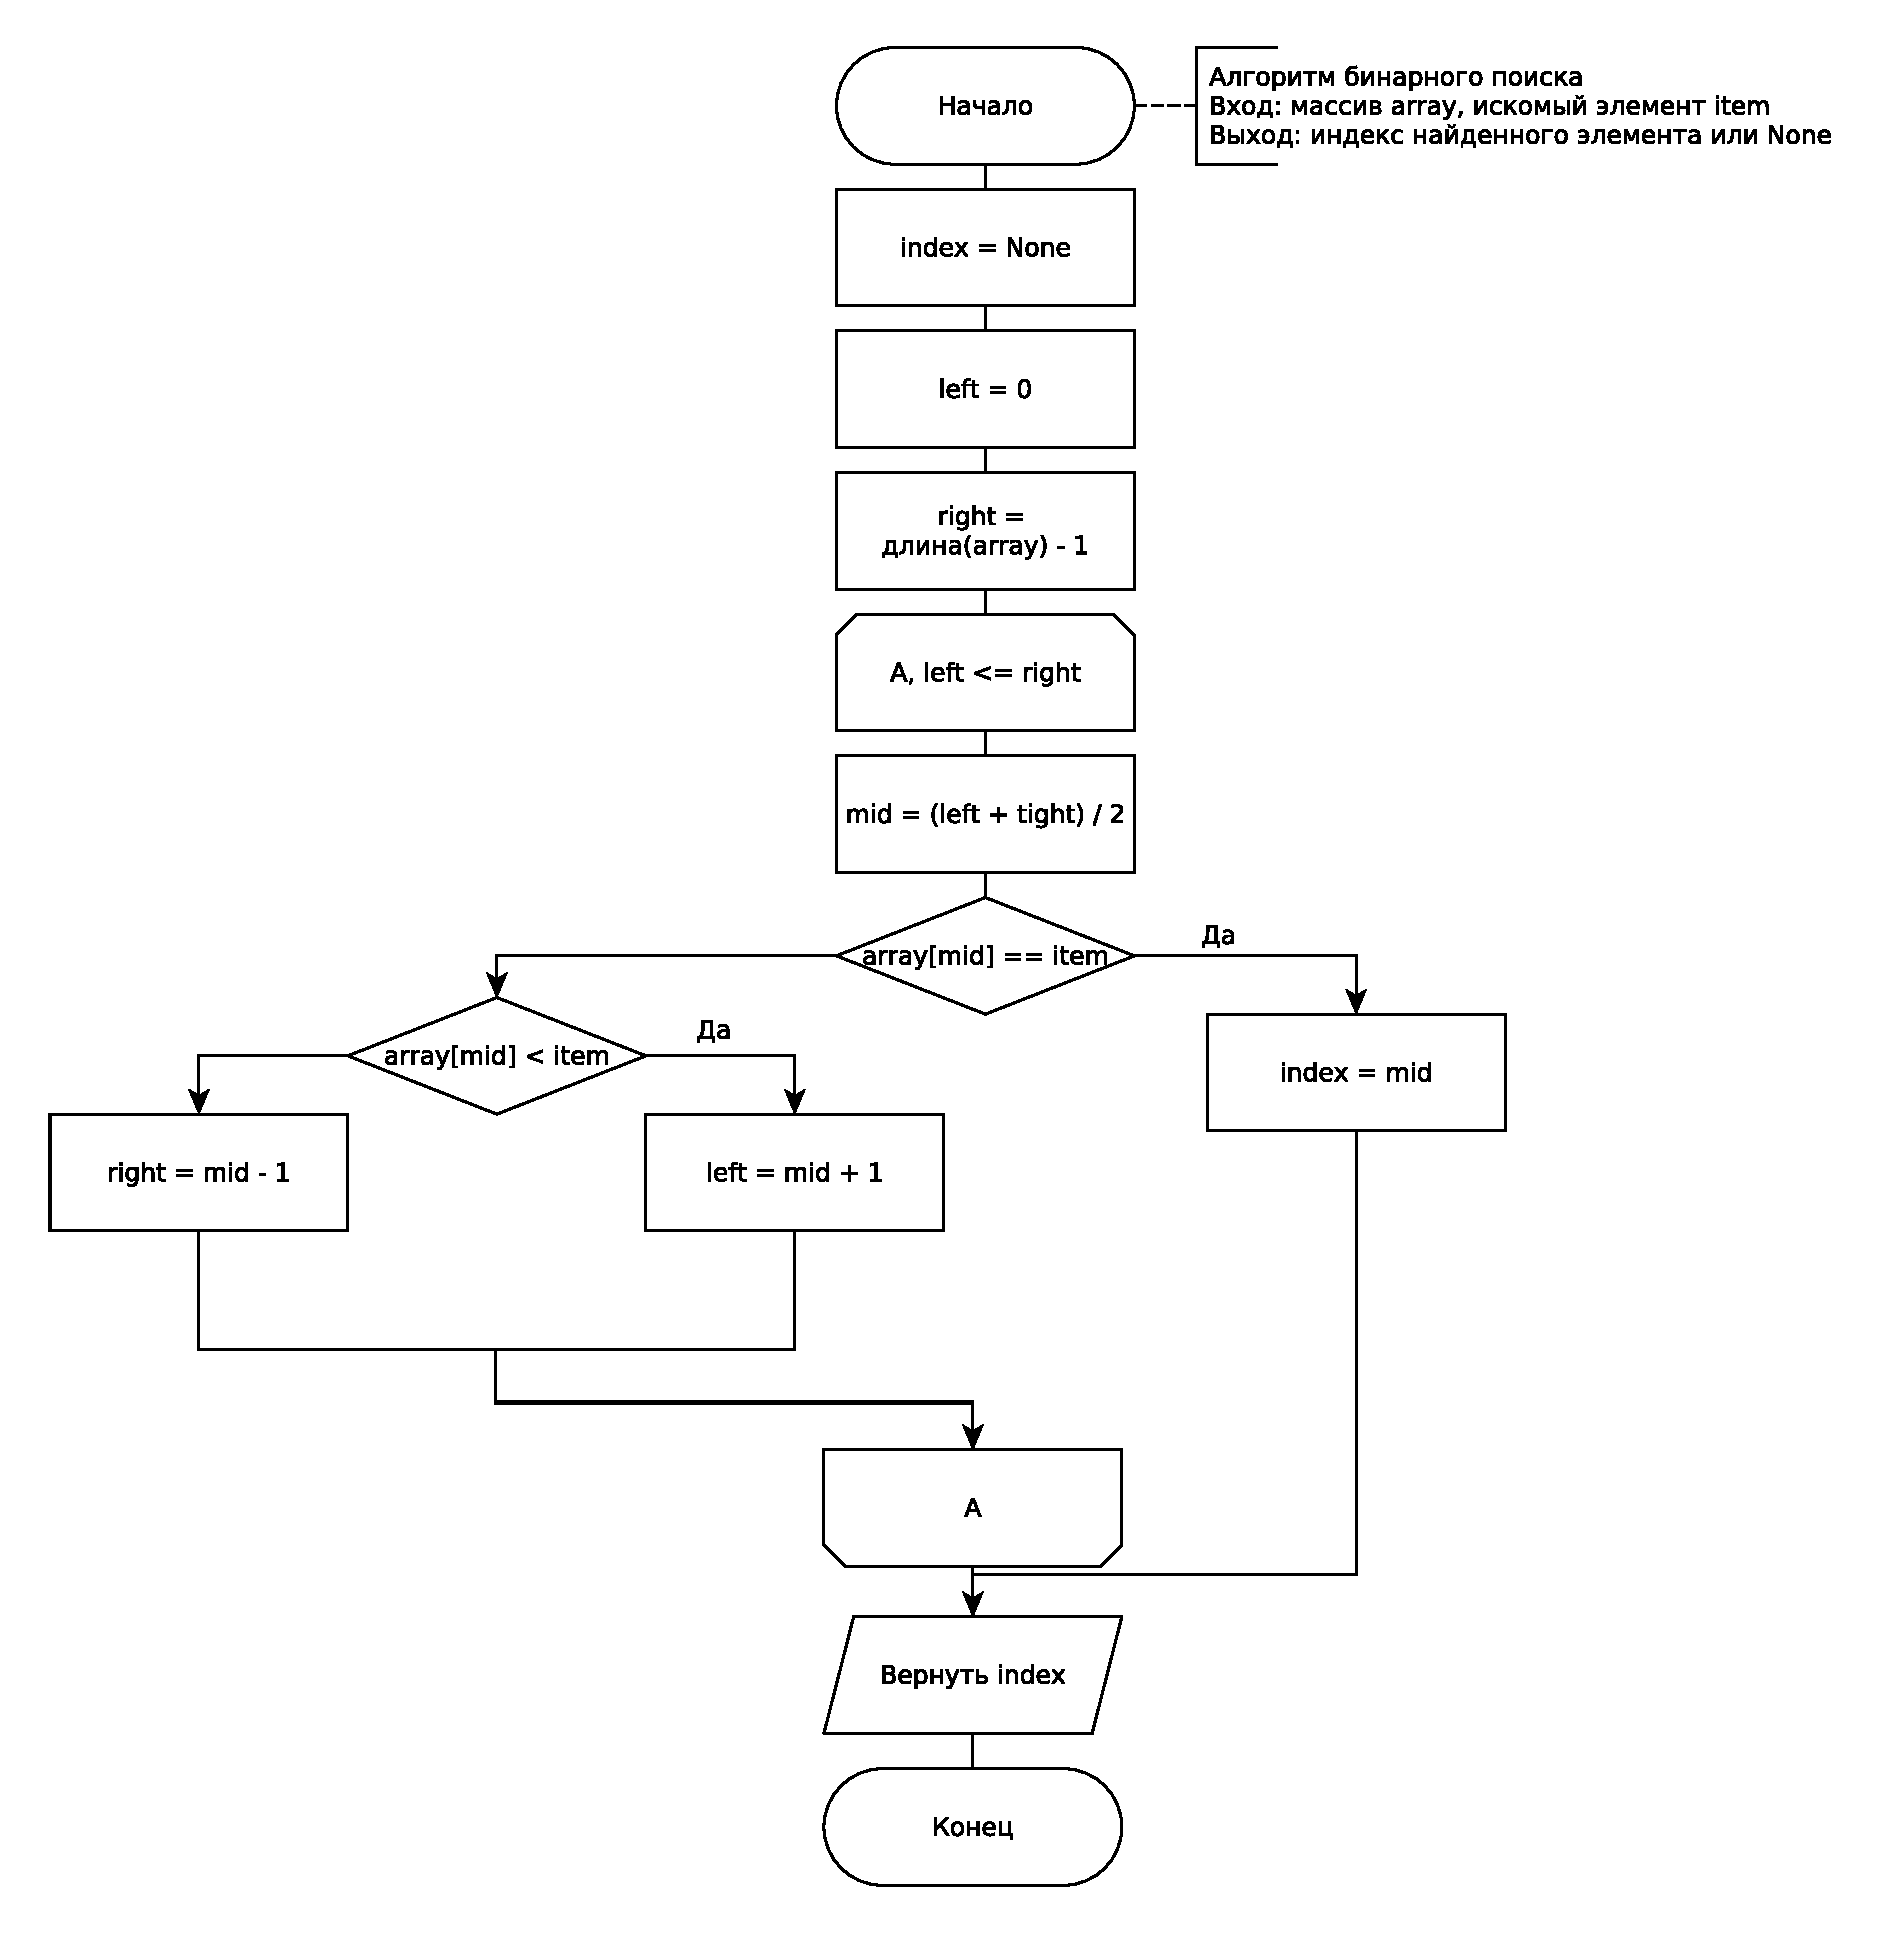
\includegraphics[scale=0.5]{img/binary_search.eps}
	\caption{Схема алгоритма бинарного поиска в массиве}
	\label{fig:Binary}
\end{figure}

\clearpage

\textbf{ВЫВОД}

 В данном разделе были представлены схемы алгоритмов поиска заданного элемента в массиве методом линейного поиска и методом бинарного поиска.

\clearpage